\typeout{************************************************}
\typeout{Chapter 1 Functions}
\typeout{************************************************}
%
\chapter{Functions}\label{}
%
\minitoc
%
\typeout{************************************************}
\typeout{Section 1.1 The Basics of Function Vocabulary}
\typeout{************************************************}
%
\section{The Basics of Function Vocabulary}\label{}
%
\begin{outcomes}
\begin{outcomelist}
\item You will understand the definition of a function.%
\item You will be able to use standard notation for functions
	                correctly, and recognize when notation has been used incorrectly.%
\item You will recognize some everyday examples of functions.%
\end{outcomelist}
\end{outcomes}
Most of us are familiar with the $\sqrt{\phantom{x}}$ symbol.
		This symbols is used to turn numbers into their square roots. Sometimes it's
		simple to do this on paper or in our heads, and sometimes it helps a lot to
		have a calculator. We can see some calculations in \cref{fun-tab-squareroots}.
%
\begin{margintable}\centering
\captionof{table}{Values of $\sqrt{x}$}
\label{fun-tab-squareroots}
\begin{tabular}{r@{}c@{}l}
\beforeheading 
\afterheading 
$\sqrt{\num{9}}$&${}={}$&\num{3}\\\normalline
$\sqrt{\num{1/4}}$&${}={}$&\num{1/2}\\\normalline
$\sqrt{\num{2}}$&${}\approx{}$&\num{1.41}\ldots\\\lastline
\end{tabular}
\end{margintable}
%
\par The $\sqrt{\phantom{x}}$ symbol represents a \emph{process}; it's a way for us to
		turn numbers into other numbers. This idea of finding some numbers based on other numbers is
		fundamental to science and mathematics that use college-level algebra. 
%
\begin{definition}[Function]\label{}
A function is a process for turning numbers into (potentially) different numbers. 
			It's important that any input consistently produces the same output.\end{definition}
%
\par This definition is so broad that you probably use functions all the time.
%
\begin{example}\label{}
Think about each of these examples. How do they fit the defintion of a function?
%
\begin{itemize}
\item If you use the year a person was born to determine how old they are, you are using a function.%
\item If you look up the Kelly Blue Book value of a Mazda Proteg\'{ e} based on how old it is, 
				you are using a function.%
\item If you use the the amount of money that you have on you to determine how many beers you could buy for 
				your friends at the bar, you are using a function.%
\end{itemize}
%
\end{example}
%
\par The process of using $\sqrt{\phantom{x}}$ to change numbers might feel more ``mathematical''
		than these examples. Let's continue thinking about $\sqrt{\phantom{x}}$ for now, since
		it's a formula-like symbol that we are familiar with. Even though we live in the age of computers,
		this symbol is not found on most
		keyboards. This doesn't stop people from using computers to calculate square roots though. Computer
		technicians write $\sq[(]$ when they want to compute a square root, as we see in \cref{fun-tab-sqrts}.
%
\begin{margintable}\centering
\captionof{table}{Values of $\sq[x]$}
\label{fun-tab-sqrts}
\begin{tabular}{r@{}c@{}l}
\beforeheading 
\afterheading 
$\sq[\num{9}]$&${}={}$&\num{3}\\\normalline
$\sq\left(\num{1/4}\right)$&${}={}$&\num{1/2}\\\normalline
$\sq[\num{2}]$&${}\approx{}$&\num{1.41}\ldots\\\lastline
\end{tabular}
\end{margintable}
%
\par The parentheses in $\sq[(]$ are very important. To see why, try to put yourself in the
          ``mind'' of a computer, and look closely at $\sq\num{16}$. The computer will recognize $\sq$
		and know that it needs to compute a square root. But computers are very picky with how they interpret input, and 
		they might not see the entire number \num{16}. A computer might read as far as $\sq\num{1}$ and think that it needs to compute this.
		That would leave $1$ with a ``6'' character still hanging. The final result would be \num{16}, and we know we inteded the  
		result to be $4$. And so the purpose of the parentheses in $\sq[\num{16}]$ is 
		to denote exactly what number needs to be operated on.
%
\par This use of $\sq[(]$ serves as a model for the standard notation that is used all over the world to
        	write down most functions. By having a standard notation for communicating about functions,
        	people in China, Venezuela, Senegal, and the United States can all communicate mathematics
        	with each other more easily.
%
\par Functions have their own names. We've seen a function named $\sq$, but any name you can
        	imagine is allowable. In the sciences, it is common to name functions with whole words,
        	like $\operatorname{weight}$ or $\operatorname{health\_index}$. In mathematics, we often
            abbreviate such function names to $w$ or $h$. And of course, since the word ``function''
            starts with ``f'', we will often name a function $f$.
%
\par It's crucial to continue reminding ourselves that functions are \emph{processes} for
        	changing numbers; they are not numbers themselves. And that means that we have a potential
        	for confusion that we need to stay aware of. In some contexts, the symbol $t$ might
        	represent a variablea number that is represented by a letter. For example, it might represent 
		how much time has passed since something started. But in other contexts, $t$
        	might represent a functiona process for changing numbers into other numbers. For example, if you 
		have a year in mind, $t$ might be the function that tells you how many tornadoes there were that year. 
		So $t$ would be a process for turning years into numbers of tornadoes. By
        	staying conscious of the context of an investigation, we avoid confusion.
%
\par Next we need to discuss how we go about using a function's name.
%
\begin{specialnote}[Function notation]
The standard notation for referring to functions involves giving the function itself a name, and then writing
			\begin{displaymath}\begin{array}{cc}
                                \text{name}\\
                                \text{of}\\
                                \text{function}
                        \end{array}
                        \left(
                        \begin{array}{cc}
                                \\
                                \text{input}\\
                                \\
                        \end{array}\right)\end{displaymath}\end{specialnote}
%
\begin{example}\label{}
$f(\num{13})$ is pronounced ``f of 13''. The word ``of'' is very important,
        		because it reminds us that $f$ is a process and we are about to apply that
        		process to the input value \num{13}. So $f$ is the function, \num{13} is the
        		input, and $f(\num{13})$ is the output we'd get from using \num{13} as input.
%
\par $f(x)$ is pronounced ``f of x''. This is just like the previous example,
        		except that the input is not some specific number. The value of $x$ could be
        		\num{13} or any other number. Whatever $x$'s value, $f(x)$ means the corresponding
        		output from the function $f$.
%
\par $\operatorname{BudgetDeficit}(2009)$ is pronounced ``BudgetDeficit of 2009''.
        		This is probably a function that takes a year as input, and gives that
        		year's federal budget deficit as output. The process here of changing a year
        		into a dollar amount might not involve any mathematical formula, but rather
        		looking up information from the Congressional Budget Office's website.
%
\par $\operatorname{Celsius}(F)$ is pronounced ``Celsius of F''. This is probably
        		a function that takes a Fahrenheit temperature as input and gives the
        		corresponding Celsius temperature as output. Maybe a formula is used to do this;
        		maybe a chart or some other tool is used to do this. Here, $\operatorname{Celsius}$
        		is the function, $F$ is the input variable, and $\operatorname{Celsius}(F)$ is the output from the function.
%
\end{example}
%
\begin{specialnote}[Function notation (continued)]
While a function has a name like $f$, and the input to that function often
                	has a variable name like $x$, the expression $f(x)$ represents the output of
                	the function. To be clear, $f(x)$ is \emph{not} a function. Rather, $f$ is a
                	function, and $f(x)$ its the output when the number $x$ is used as input.\end{specialnote}
%
\par As mentioned earlier, we need to remain conscious of the context of any symbol we
       		are using. It's possible for $f$ to represent a function (a process), but it's also
       		possible for $f$ to represent a variable (a number). Similarly, parentheses might
       		indicate the input of a function, or they might indicate that two numbers need to
       		be multiplied. It's up to our judgment to interpret mathematical expressions in the
       		right context. Consider the expression $a(b)$. This could easily mean the output of
       		a function $a$ with input $b$. It could also mean that two numbers $a$ and $b$ need
       		to be multiplied. It all depends on the context in which these symbols are being used.
%
\begin{checkpoint}
\begin{problem}\label{}
Describe your own example of a function using experience from your life. You will need some 
                    kind of input variable, like ``number of years since 2000'' or ``weight of a bowling ball''. You will 
				need a process for turning that number into a different kind of number. The process does not need to
                		involve a formula; a verbal description would be fine.
%
\par Give your function a name. Write the symbol that you would use to represent
                		input. Write the symbol(s) that you would use to represent output.
%
\begin{longsolution}
%
Answers will vary.
%
\end{longsolution}
%
\begin{shortsolution}
%
Answers will vary.
%
\end{shortsolution}
%
\end{problem}
%
\end{checkpoint}
%
\par Sometimes it's helpful to think of a function as a machine.
%
\par This illustrates how complicated functions are. A number is just a number. But a function has the capacity to 
		take in all kinds of different numbers into it's hopper (feeding tray) and do different things to each of them. So
		functions are complicated.
%
\typeout{************************************************}
\typeout{Subsection 1.1.1 Tables and Graphs}
\typeout{************************************************}
%
\subsection{Tables and Graphs}\label{}
%
Since functions are potentially so complicated, we seek out new ways to understand
        		them better. Two basic tools for understanding a function better are tables and graphs.
%
\begin{example}\label{fun-ex-BudgetDeficit}
Consider the function $\operatorname{BudgetDeficit}$, that takes in a year as
        			its input and outputs the US federal budget deficit for that year. For example,
        			the Congressional Budget Office's website tells us that
        			$\operatorname{BudgetDeficit}(2009)$ is $\SI{1.41}[\$]{\trillion}$. If we'd like
        			to understand this function better, we might make a table of all the inputs and
        			outputs we can find. Using the CBO's 
				website\footnote{\href{http://data.bls.gov/timeseries/LNS14000000}{Congressional Budget Office}}, we put together 
				\cref{fun-tab-BudgetDeficit}.
%
\begin{table}[thb]\centering
\caption{}
\label{fun-tab-BudgetDeficit}
\begin{tabular}{S[table-format=4.0]S[table-format=1.2]}
\beforeheading 
\heading{input}&\heading{output}\\\normalline
\heading{$x$ (year)}&\heading{$\operatorname{BudgetDeficit}(x)$ ($\si{\$\trillion}$)}\\\normalline
\afterheading 
2007&0.16\\\normalline
2008&0.46\\\normalline
2009&1.41\\\normalline
2010&1.29\\\normalline
2011&1.30\\\lastline
\end{tabular}
\end{table}
%
\par How is this table helpful? There are things about the function that we can see now by looking at the numbers in this table.
%
\begin{itemize}
\item We can see that the budget deficit has grown by quite a bit over the entire five-year period.%
\item We can see that there was a particularly large jump in 2008.%
\item We can see that the deficit reduced by a little bit between 2009 and 2010, and then remained stable.%
\end{itemize}
%
\par These observations serve to help us understand the function $\operatorname{BudgetDeficit}$ a little better.
%
\end{example}
%
\begin{example}\label{fun-ex-sqrttable}
Let's return to our example of the function $\sq$. Tabulating some inputs and outputs reveals \cref{fun-tab-sqrtexample}.
%
\begin{table}[thb]\centering
\caption{}
\label{fun-tab-sqrtexample}
\begin{tabular}{S[table-format=1.0]c}
\beforeheading 
\heading{input}&\heading{output}\\\normalline
\heading{$x$}&\heading{$\sq[x]$}\\\lastline
\afterheading 
0&\num{0}\\\normalline
1&\num{1}\\\normalline
2&$\approx\num{1.41}$\\\normalline
3&$\approx\num{1.73}$\\\normalline
4&\num{2}\\\lastline
\end{tabular}
\end{table}
%
\par How is this table helpful? Here are some observations that we can make now.
%
\begin{itemize}
\item We can see that when input numbers increase, so do output numbers.%
\item We can see even though outputs are increasing, they increase by less and less with each step forward in $x$.%
\end{itemize}
%
\par These observations help us understand $\sq$ a little better. For instance, based on these observations which do you think is larger: 
				the difference between $\sq[23]$ and $\sq[24]$, or the difference between $\sq[24]$ and $\sq[25]$?
%
\end{example}
%
\par Another powerful tool for understanding functions better is a graph.
        		Given a function $f$, one way to make its graph is to take a table of input and
        		output values, and read each row as the coordinates of a point in the $xy$-plane.
%
\begin{example}\label{fun-ex-budgetgraph}
Returning to the function $\operatorname{BudgetDeficit}$ that we studied in \cref{fun-ex-BudgetDeficit}, in order to make a 
				graph of this function we view \cref{fun-ex-BudgetDeficit} as a list of points with $x$ and $y$ coordinates, as in 
				\cref{fun-tab-BudgetDeficitCoords}. We then plot these points on a set of coordinate axes, as in \cref{fun-fig-BudgetDeficit}. 
				The points have been connected with a curve so that we can see the overall pattern given by the progression of points.
        			Since there was not any actual data for inputs in between any two years, the curve is dashed. In other words, this curve is dashed because 
				it just represents someone's best guess as to how to connect the plotted points. Only the plotted points themselves are precise.
%
\begin{table}[thb]\centering
\caption{}
\label{fun-tab-BudgetDeficitCoords}
\begin{tabular}{*{1}{c}}
\beforeheading 
(input, output)\\\normalline
$(x,\operatorname{BudgetDeficit}(x))$\\\lastline
\afterheading 
$(2007, 0.16)$\\\normalline
$(2008, 0.46)$\\\normalline
$(2009, 1.41)$\\\normalline
$(2010, 1.30)$\\\normalline
$(2011, 1.29)$\\\lastline
\end{tabular}
\end{table}
%
\par How has this graph helped us to understand the function better? All of the observations that we made in \cref{fun-ex-BudgetDeficit} are perhaps even
        			more clear now. For instance, the spike in the deficit between 2008 and 2009 is now visually apparent. Seeking an explanation for this spike, we recall
        			that there was a financial crisis in late 2008. Revenue from income taxes dropped at the same time that federal money was spent to prevent further losses.
%
\end{example}
%
\begin{example}\label{fun-ex-sqrtgraph}
Now let's construct a graph for $\sq$. Tabulating inputs and outputs gives the points in \cref{fun-tab-sqrtCoords}, which in turn gives us the 
				graph in \cref{fun-fig-sqrt}.
%
\begin{table}[thb]\centering
\caption{}
\label{fun-tab-sqrtCoords}
\begin{tabular}{*{1}{c}}
\beforeheading 
(input, output)\\\normalline
$(x,\sq(x))$\\\lastline
\afterheading 
$(0,0)$\\\normalline
$(1,1)$\\\normalline
$\approx(2,1.41)$\\\normalline
$\approx(3,1.73)$\\\normalline
$(4,2)$\\\lastline
\end{tabular}
\end{table}
%
\par Just as in the previous example, we've plotted points where we have concrete coordinates, and then we have made our best attempt to connect those points
        			with a curve. Unlike the previous example, here we believe that points could continue to be computed and plotted indefinitely to the right, and so we
        			have added an arrowhead to the graph.
%
\par What has this graph done to improve our understanding of $\sq$?  As inputs ($x$-values) increase, the outputs ($y$-values) increase too, 
				although not at the same rate. In fact we can see that our graph is steep on its left, and less steep as we move to the right. This confirms our earlier 
				observation in \cref{fun-ex-sqrttable} that outputs increase by smaller and smaller amounts as the input increases.
%
\end{example}
%
\begin{specialnote}[The graph of a function]
Given a function $f$, when we refer to a \emph{graph of $f$} we are \emph{not} referring to an entire picture, like 
				\cref{fun-fig-sqrt}. A graph of $f$ is only \emph{part} of that picture: the curve and the points that it connects.
				Everything else: axes, tick marks, the grid, labels, and the surrounding white space is just useful decoration, so that we can read the graph more easily.
%
\par It is also common to refer to the graph of $f$ as the graph of the \emph{equation} $y=f(x)$. However we should never refer to ``the graph of $f(x)$''.
				That would indicate a fundamental misunderstanding of our notation. We have decided that $f(x)$ is the output for a certain input $x$. That means that 
				$f(x)$ is just a number; a relatively uninteresting thing compared to $f$ the function, and not worthy of any two-dimensional picture.
%
\end{specialnote}
%
\par While it is important to be able to make a graph of a function $f$, we also need to be capable of looking at a graph and reading it well. 
			A graph of $f$ provides us with helpful specific information about $f$; it tells us what $f$ does to its input values. When we were making graphs, 
			we plotted points of the form \begin{displaymath}(\text{input},\text{output})\text{.}\end{displaymath} Now given a graph of $f$, we interpret coordinates in the same way.
%
\begin{figure}[!htbp]
\centering

                    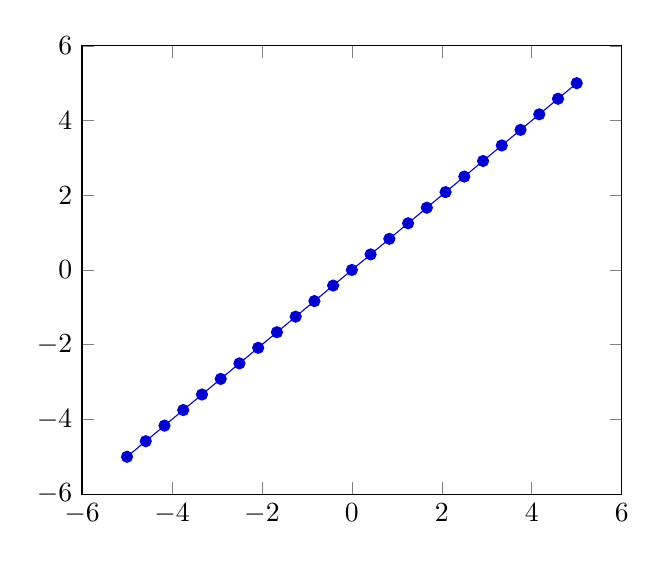
\begin{tikzpicture}
                        \begin{axis}
                        \addplot{x};
                        \end{axis}
                    \end{tikzpicture}
                  \caption{caption text goes here\label{fun-fig-readgraph}}
\end{figure}
%
\begin{figure}[!htbp]
\centering

                    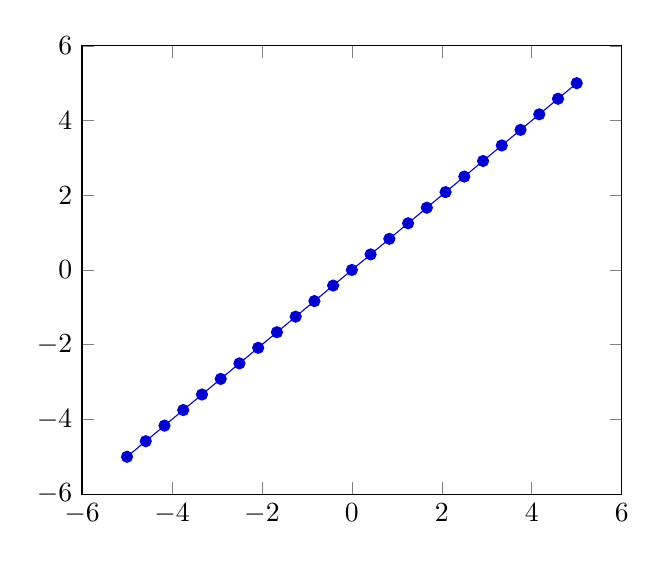
\begin{tikzpicture}
                        \begin{axis}
                        \addplot{x};
                        \end{axis}
                    \end{tikzpicture}
                  \caption{caption text goes here\label{}}
\end{figure}
%
\par In \cref{fun-fig-readgraph} we have a graph of a function $f$. If we wish to find $f(1)$, we recognize that \num{1} is being used as an input.
			So we would want to find a point of the form $(1,\phantom{y})$. Seeking out $x$-coordinate \num{1} in \cref{fun-fig-readgraph}, we find that 
			the only such point is $(1,2)$. Therefore the output for \num{1} is \num{2}; in other words $f(1)=2$.
%
\begin{checkpoint}
\begin{problem}\label{}
Use the graph of $f$ in \cref{fun-fig-readgraph} to find $f(0)$, $f(3)$, and $f(4)$.
%
\begin{longsolution}
%
 To find $f(0)$, locate $0$ on the $x$-axis. Moving up or down from there, the only place you can meet the graph
					of $f$ is at $(0,0.5)$. So $f(0)=0.5$.
%
\par  To find $f(3)$, locate $3$ on the $x$-axis. Moving up or down from there, the only place you can meet the graph
                                        of $f$ is at $(3,3)$. So $f(3)=3$.
%
\par  To find $f(4)$, locate $4$ on the $x$-axis. Moving up or down from there, the only place you can meet the graph
                                        of $f$ is at $(4,2)$. So $f(4)=2$.
%

%
\end{longsolution}
%
\begin{shortsolution}
%
$f(0)=0.5$, $f(3)=3$, and $f(4)=2$
					
%
\end{shortsolution}
%
\end{problem}
%
\end{checkpoint}
%
\typeout{************************************************}
\typeout{Section 1.2 foo}
\typeout{************************************************}
%
\section{foo}\label{}
%
here is another section
%
\typeout{************************************************}
\typeout{Section 1.3 bar}
\typeout{************************************************}
%
\section{bar}\label{}
%
here is another section
%
\typeout{************************************************}
\typeout{Chapter 2 Exponential functions}
\typeout{************************************************}
%
\chapter{Exponential functions}\label{}
%
\begin{comment}
This file was created using ./xsl/omd2tex.xsl,
there is no point in editing it :)

This file is all about exponential functions.
\end{comment}

\typeout{************************************************}
\typeout{Section 2.1 Introduction}
\typeout{************************************************}
%
\section{Introduction}\label{firstsection}
%
\begin{outcomes}
\begin{outcomelist}
\item  Explore increasing and decreasing functions, particularly in the context of concavity;%
\item  Determine a function's concavity based on a table of values, a graph, or a description. %
\end{outcomelist}
\end{outcomes}

In our mathematical adventures so far we have studied linear, quadratic, 
and radical functions. The simplicity of these functions is useful when 
introducing new concepts such as transformations, composition, and 
inverse functions; but it is somewhat restrictive when we wish to 
consider interesting real-world application problems. 
\cref{firstsection} 
\Cref{firstsection} 
\vref{firstsection} 
\Vref{firstsection} 

%
\par 
HERE:
\crefrange{firstsection}{secondsection} 
\Crefrange{firstsection}{secondsection}                
\vrefrange{firstsection}{secondsection}                      
\Vrefrange{firstsection}{secondsection} 
DONE

need to fix referencing so that it uses *our* ID (at the very least in the .tex version)
need to work out how to define a 'xrefRange' command (two arguments???)
  
%
\typeout{************************************************}
\typeout{Section 2.2 Method}
\typeout{************************************************}
%
\section{Method}\label{secondsection}
%
\begin{problem}\label{}
Describe your own example of a function using experience from your life. You will need some 
                    kind of input variable, like ``number of years since 2000'' or ``weight of a bowling ball''. You will 
				need a process for turning that number into a different kind of number. The process does not need to
                		involve a formula; a verbal description would be fine.
%
\par Give your function a name. Write the symbol that you would use to represent
                		input. Write the symbol(s) that you would use to represent output.
%
\begin{longsolution}
%
Answers will vary.
%
\end{longsolution}
%
\begin{shortsolution}
%
Answers will vary.
%
\end{shortsolution}
%
\end{problem}
%
\begin{definition}[Function]\label{}
A function is a process for turning numbers into (potentially) different numbers. 
			It's important that any input consistently produces the same output.\end{definition}
%
\begin{example}\label{}
Think about each of these examples. How do they fit the defintion of a function?
%
\begin{itemize}
\item If you use the year a person was born to determine how old they are, you are using a function.%
\item If you look up the Kelly Blue Book value of a Mazda Proteg\'{ e} based on how old it is, 
				you are using a function.%
\item If you use the the amount of money that you have on you to determine how many beers you could buy for 
				your friends at the bar, you are using a function.%
\end{itemize}
%
\end{example}
%
